\section{Gestion des inscriptions}

\textbf{Si vous êtes un membre du staff, et que vous avez la permission de gérer les inscriptions}, vous pouvez alors accéder à la page de gestion des inscriptions, depuis l'onglet \enquote{Staff} tout à droite du menu de navigation.

\begin{figure}[H]
\centering
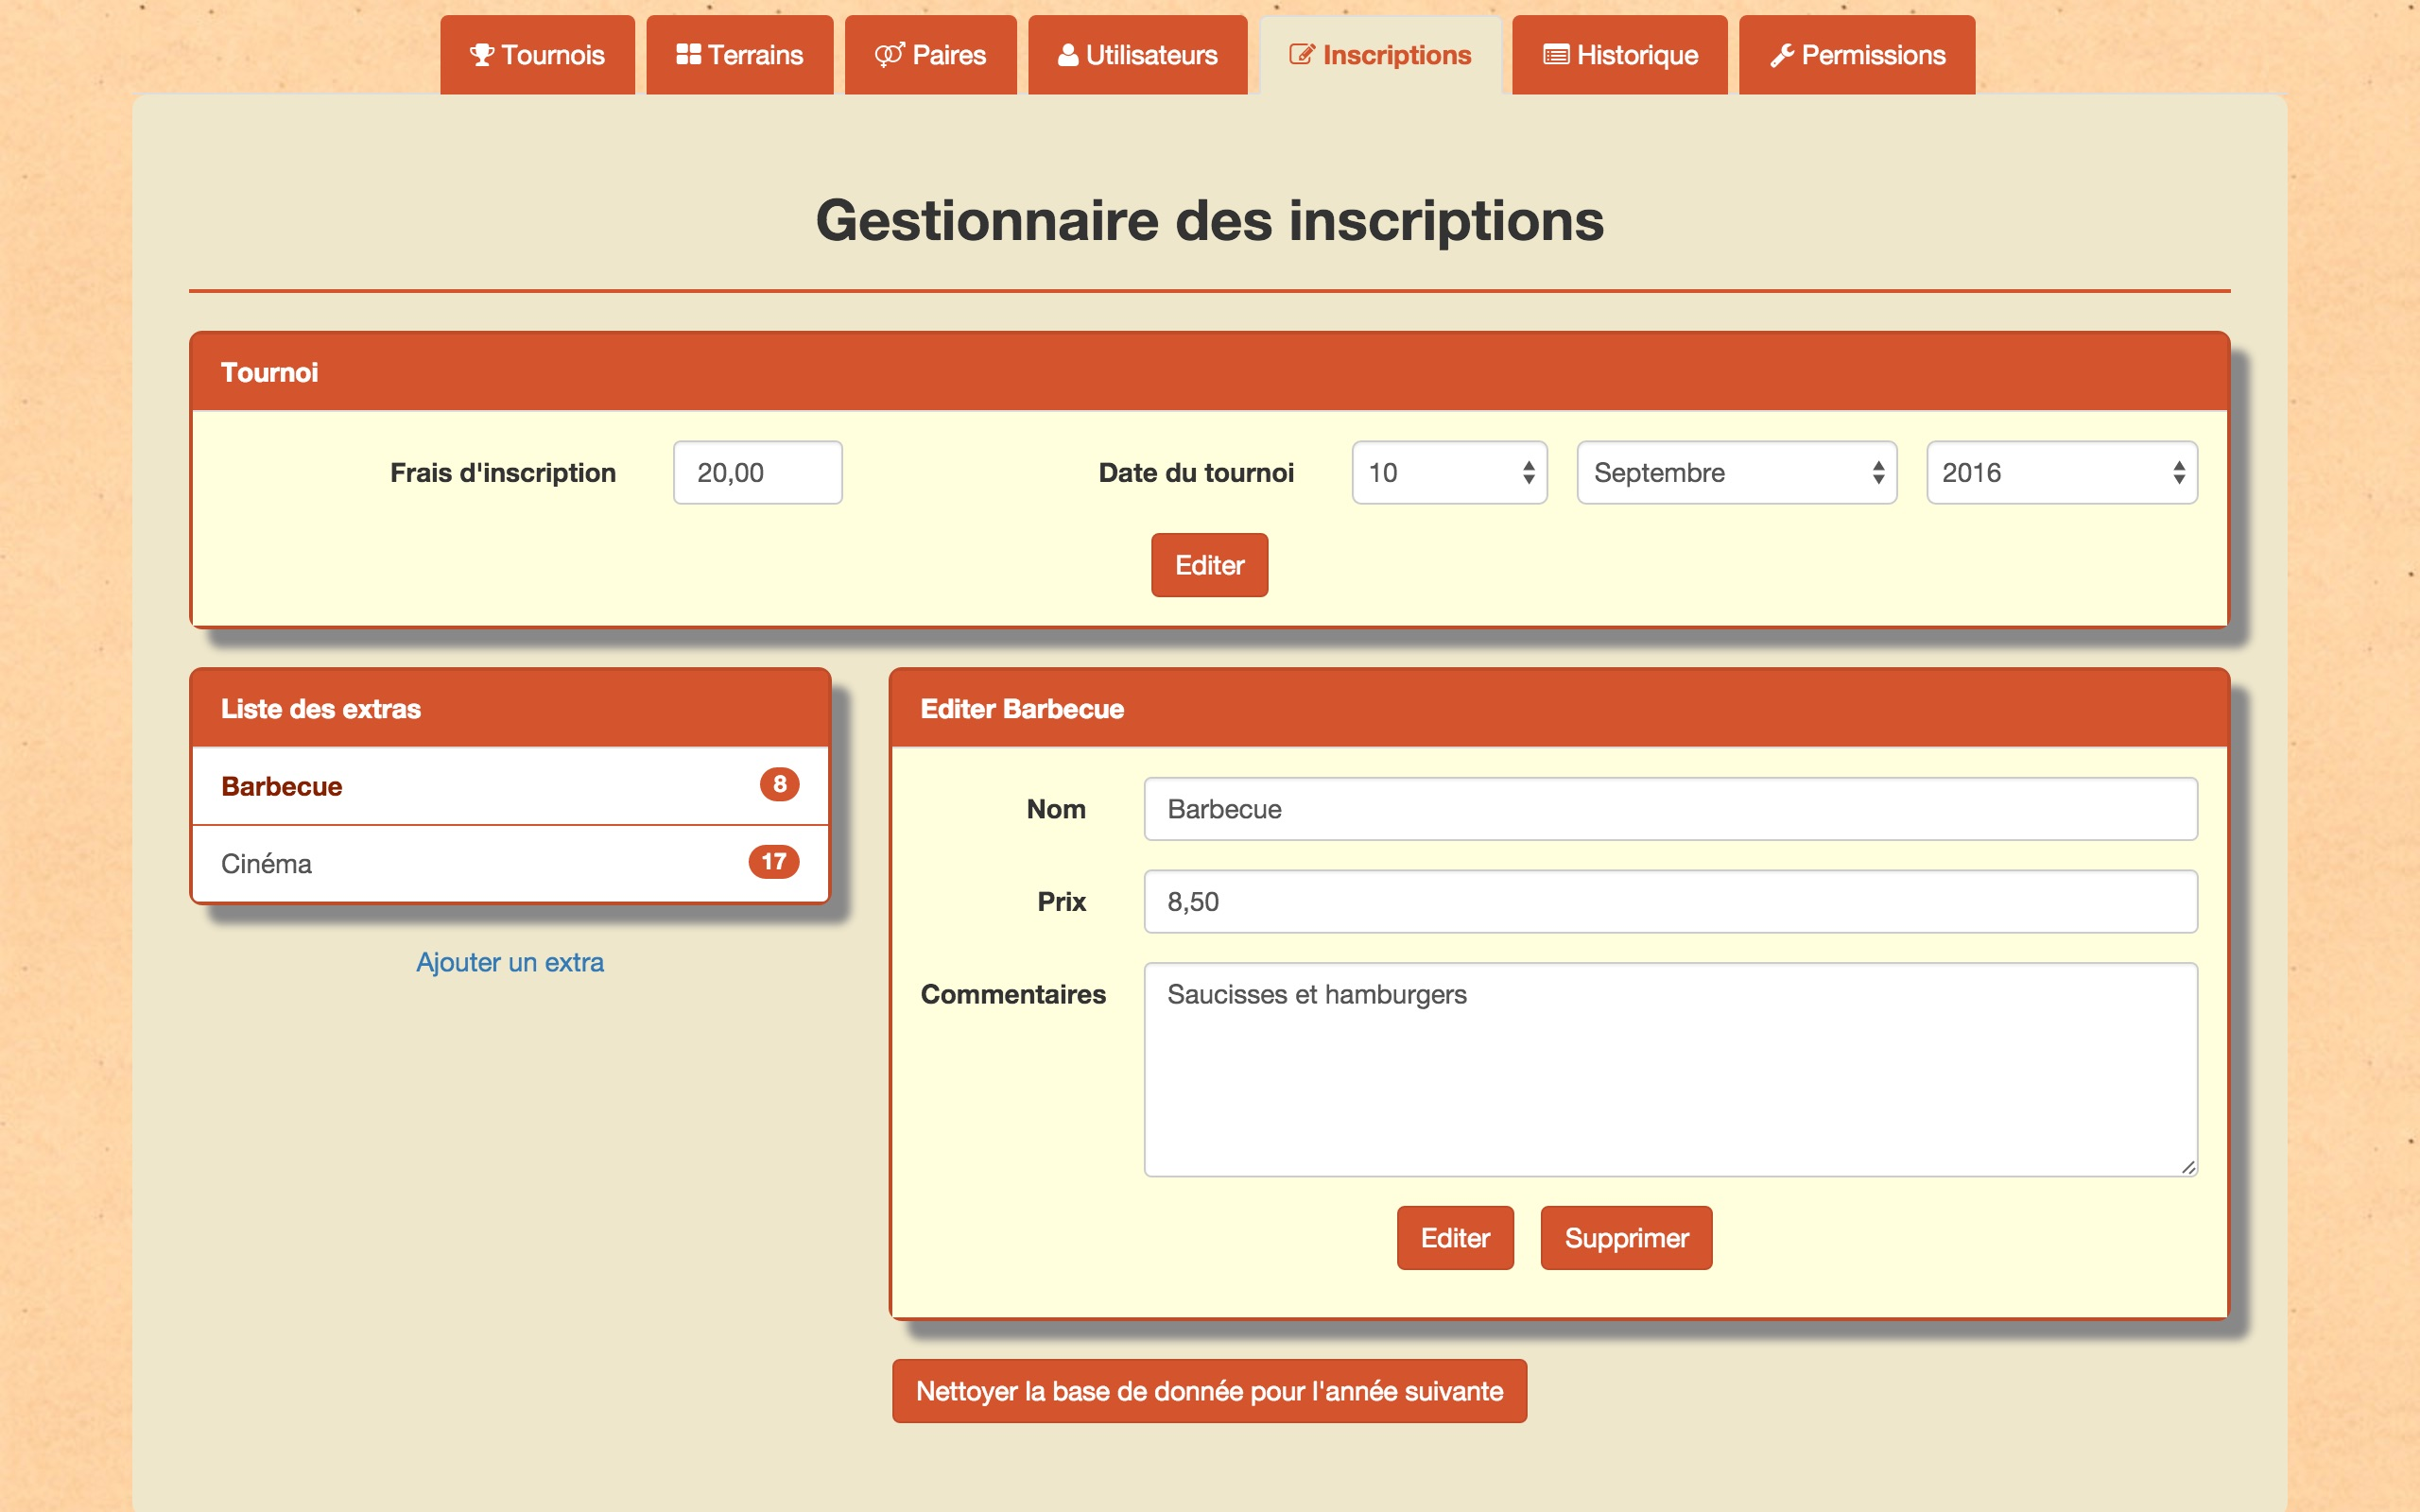
\includegraphics[scale=0.15]{gestion-inscriptions/gestion-inscriptions.jpg}
\caption{Page staff principale pour la gestion des inscriptions}
\end{figure}

Pour donner la permission à un utilisateur de gérer les paramètres des inscriptions, l'admin doit lui octroyer les permissions à partir de la page \enquote{Gestionnaire des permissions} \ref{Gestion des permissions}.\newline

Sur cette page de gestion des inscriptions, un membre du staff peut modifier les frais d'inscription, changer la date du début de l'événement, et gérer les extras lors de l'inscription à un tournoi.

\subsection{Les frais d'inscription et la date du tournoi}

Depuis la page staff \enquote{Gestionnaire des inscriptions}, vous pouvez gérer les frais des inscriptions et la date du début de l'événement \textit{Le Charles de Lorraine}. Le premier module \enquote{Tournoi} permet de faire ces modifications, en éditant les paramètres \enquote{Frais d'inscription} et \enquote{Date du tournoi}, puis en cliquant sur le bouton \textit{Editer}, toujours dans ce module.

\begin{figure}[H]
\centering
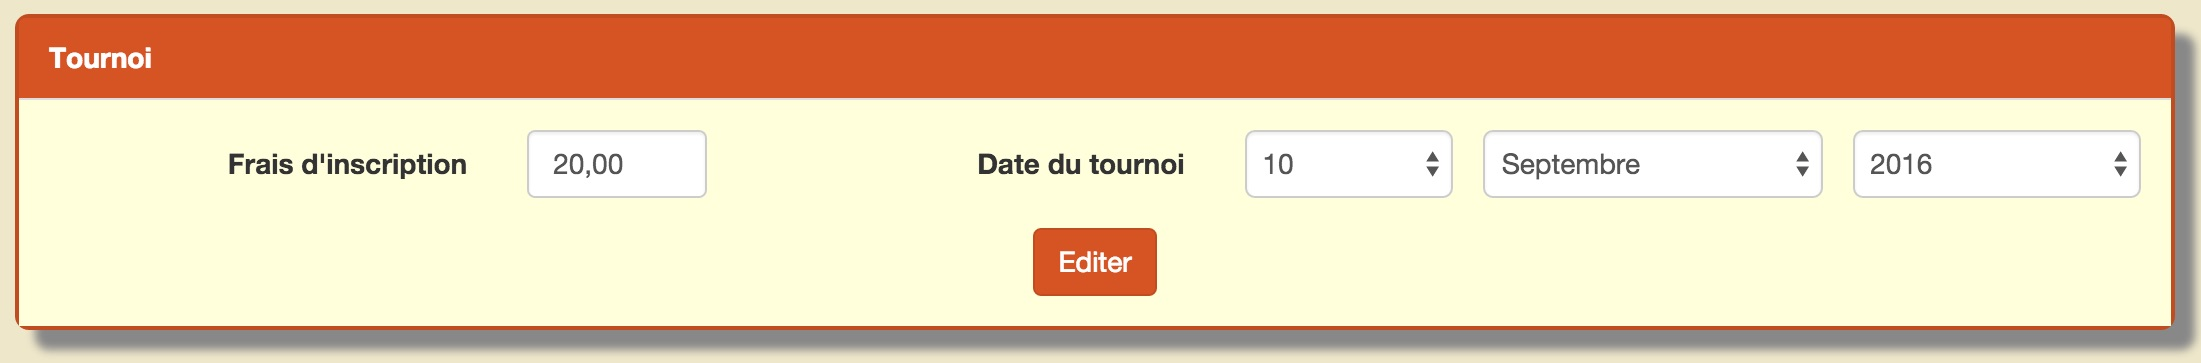
\includegraphics[scale=0.15]{gestion-inscriptions/gestion-inscriptions-tournoi.jpg}
\caption{Module de modification des frais d'inscription et de la date du début de l'événement}
\end{figure}

\subsection{Gestion des extras}

Sous le module \enquote{Tournoi}, il y a un panneau de configuration pour gérer les extras, qui permet d'ajouter des extras, de les modifier, et de les supprimer.

\begin{figure}[H]
\centering
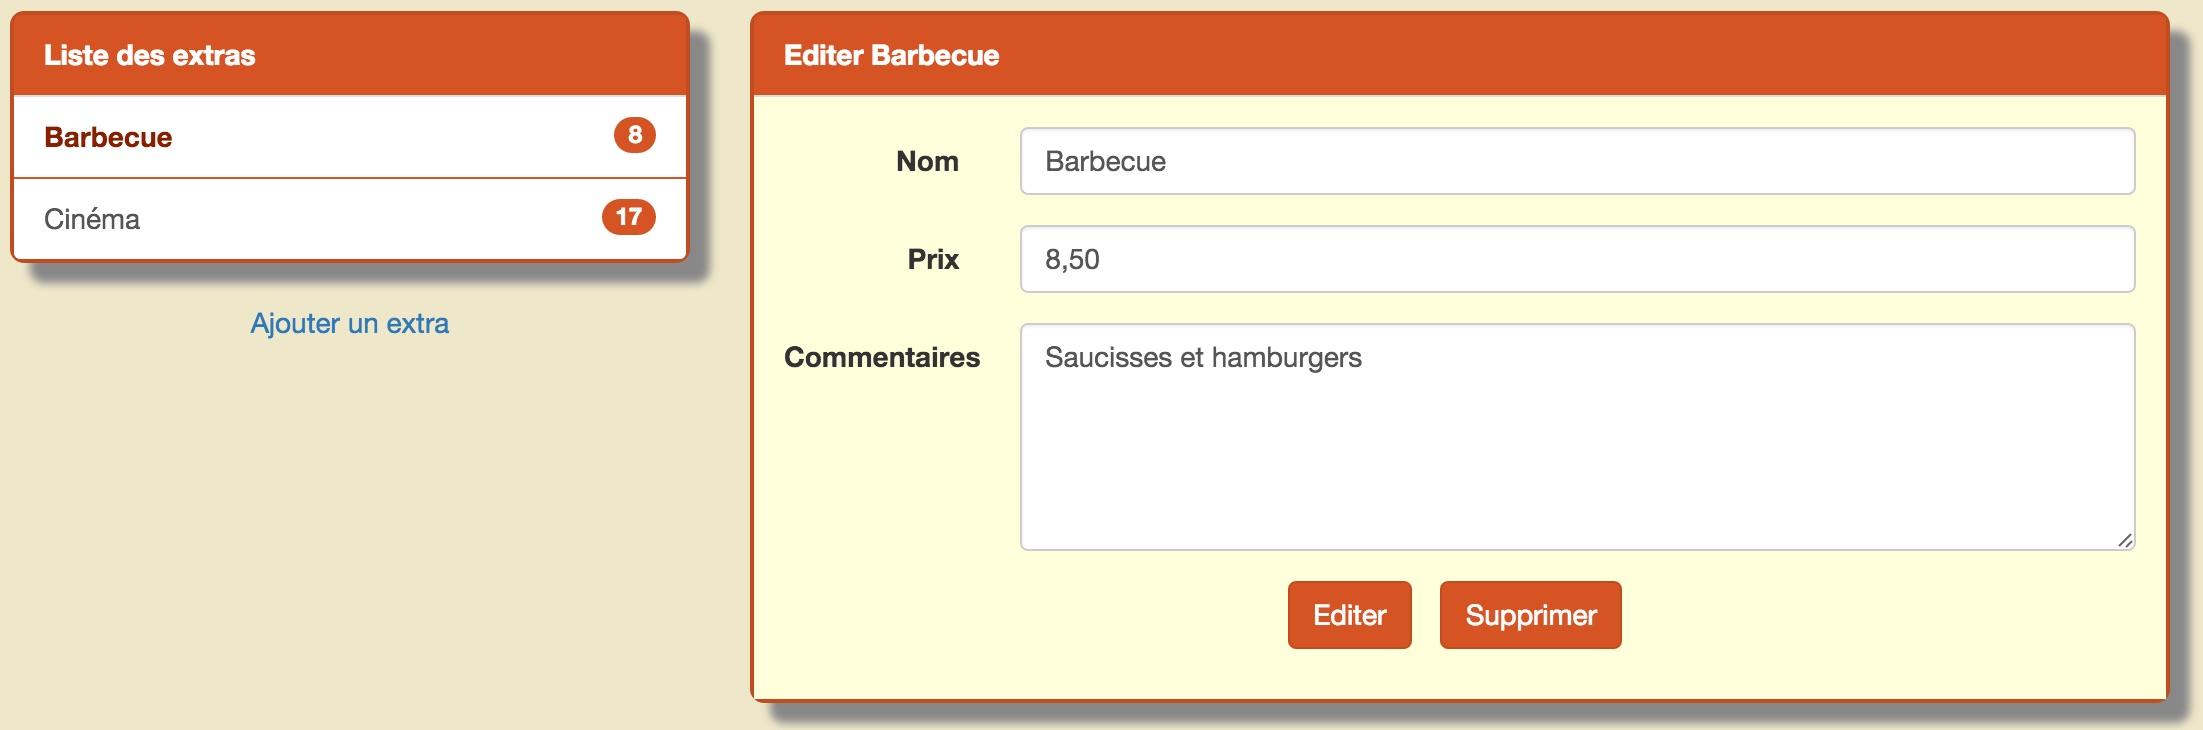
\includegraphics[scale=0.15]{gestion-inscriptions/gestion-inscriptions-extras.jpg}
\caption{Modules de gestion des extras}
\end{figure}

Le \textit{module de gauche} contient une liste de tous les extras proposés lors de l'inscription à un tournoi. Chaque extra est résumé par son nom, et un nombre encerclé à droite indiquant le nombre de personnes ayant sélectionné cet extra. L'extra actuellement sélectionné a son nom coloré en rouge. Le texte sous la liste des extra, \enquote{Ajouter un extra}, est cliquable et permet de créer un nouvel extra en remplissant le formulaire à droite juste après avoir cliqué sur le lien, puis en validant l'ajout de l'extra en cliquant sur le bouton \textit{Ajouter}.\newline

Le \textit{module de droite} s'adapte à la dernière action effectuée dans le module de gauche :

\begin{itemize}
\item \textbf{si l'utilisateur a sélectionné un extra}, alors le module de droite propose d'éditer l'extra sous forme d'un formulaire avec les champs \enquote{Nom}, \enquote{Prix}, et \enquote{Commentaires}, pré-remplis avec les informations de l'extra sélectionné. Pour confirmer l'édition de l'extra, cliquez sur le bouton \textit{Editer} en bas du module de droite. Pour supprimer l'extra, cliquez sur le bouton \textit{Supprimer} en bas du module de droite ;
\item \textbf{si l'utilisateur a cliqué sur le lien \enquote{Ajouter un extra}}, alors le module de droite propose également un formulaire, mais celui-ci est vide, les champs correspondent aux informations du nouvel extra à ajouter. Pour confirmer l'ajout de l'extra, cliquez sur le bouton \textit{Ajouter}, en bas du module de droite.
\end{itemize}
\bigskip

En ajoutant, modifiant, ou supprimant un extra, un message vert confirmera l'action effectuée.

\subsection{Préparer la base de données pour l'année suivante}

Pour préparer la base de données pour l'année suivante, l'utilisateur qui peut accéder à la page \enquote{Gestionnaire des inscriptions} peut cliquer sur le bouton \textit{Nettoyer la base de données pour l'année suivante} tout en bas de la page.\newline

Cette action implique \textbf{beaucoup de changements} dans la base de donnees :

\begin{itemize}
\item \textit{tous les tournois} sont renouvellés ;
\item \textit{toutes les paires} sont retirées de la base de données ;
\item \textit{tous les utilisateurs et terrains actuels} deviennent vétérans ;
\item \textit{tous les terrains} deviennent invalides ;
\item \textit{les informations importantes des tournois}, comme le gagnant ou les finalistes des tournois, sont indiqués sur la page des résultats, à la fin de la description de l'événement de la page d'accueil du site web ;
\item \textit{tout le reste} est inchangé
\end{itemize}
\bigskip

Étant donné que c'est une action très importante, une boîte de dialogue avec la mention \textbf{\enquote{ATTENTION !!!}} demande à l'utilisateur de confirmer son action. Cette action est irréversible !